% !TEX root=../root.tex

\subsection{Simulation}

\begin{figure}
  \centering
  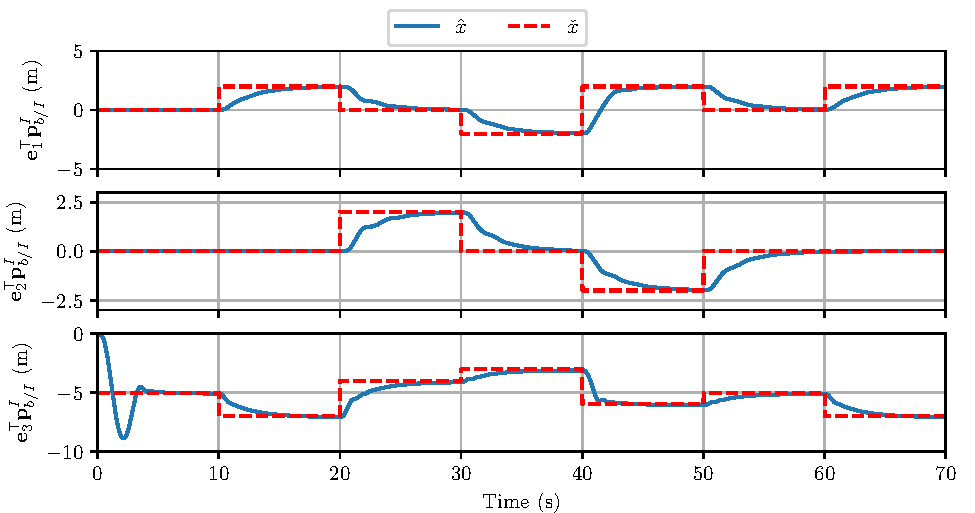
\includegraphics[width=0.4\textwidth]{figures/sim_wps_position}
  \caption[LQR Simulation Results Flying Waypoints]{Simulation results for the position of the multirotor UAV given step
  inputs to position. The red dotted line is the desired position and the blue
solid line is the estimated position.}
  \label{f:sim_wps}
\end{figure}

\begin{figure}
  \centering
  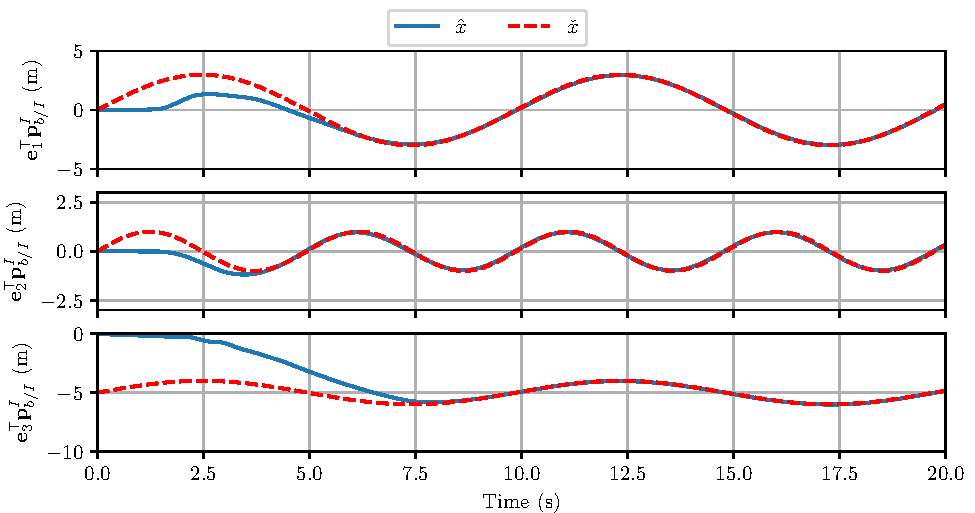
\includegraphics[width=0.4\textwidth]{figures/sim_fig8_position}
  \caption[LQR Simulation Results Flying a Trajectory]{Simulation results of a multirotor UAV tracking a figure eight
  trajectory. The red dotted line is the desired position and the blue solid
line is the estimated position.}
  \label{f:sim_fig8}
\end{figure}

Figs.~\ref{f:sim_wps} and~\ref{f:sim_fig8} show simulation results of the
controller following desired position step inputs (waypoints) and a figure-eight trajectory. The
multirotor begins the simulation at rest on the ground and converges to the
desired trajectory within a few seconds. Note that the figure-eight trajectory
tracking is near perfect even though the feed forward inputs computed
from~\eqref{eq:traj_p} -~\eqref{eq:traj_omega} do not account for the force due to drag and
the controller does not model thrust dynamics nor torque dynamics.
